\lecture{9}{3 Nov.}{}

\subsection{The Threshold for Containing \texorpdfstring{\(H\)}{H}}

We answer \autoref{q:subgraph-converse} for strictly balanced \(H\) (\autoref{def:balanced}); for those, \(m(H) = \frac{e(H)}{v(H)}\), so the threshold is the first-moment guess \(n^{-v(H)/e(H)}\).

\begin{theorem}\label{thm:subgraph-threshold}
    Let \(H\) be strictly balanced with \(e(H) \ge 1\). Then
    \[
        p^{*} = n^{-\frac{1}{m(H)}} = n^{-\frac{v(H)}{e(H)}}
    \]
    is a threshold for \(H \subseteq G(n,p)\). Moreover, if \(p \gg p^{*}\), then \(X_H = (1+o(1))\,\mathbb{E}[X_H] \to \infty\) with high probability. For \(H = K_k\), which is strictly balanced, this is \autoref{thm:clique-threshold}.
\end{theorem}

\begin{proof}
    Write \(v = v(H)\), \(e = e(H)\). Since \(H\) is balanced, \(m(H) = \frac{e}{v}\), which gives the second expression for \(p^{*}\).

    \emph{Setup.} Enumerate the copies of \(H\) in \(K_n\) as \(H_1, \ldots, H_M\). By \autoref{lem:count-copies},
    \[
        M = \frac{n(n-1)\cdots(n-v+1)}{\abs{\mathrm{Aut}(H)}} \le n^{v}
        \qquad\text{and}\qquad
        M = \Theta\bigl( n^{v} \bigr).
    \]
    Let \(E_i \coloneqq \{H_i \subseteq G(n,p)\}\). The \(e\) edges of \(H_i\) are present independently with probability \(p\) each, so \(\mathbb{P}(E_i) = p^{e}\). Since \(X_H = \sum_{i=1}^{M} \mathbbm{1}_{E_i}\), \autoref{thm:linearity} gives
    \begin{equation}\label{eq:subgraph-mean-M}
        \mathbb{E}[X_H] = \mathbb{E}\Bigl[ \sum_{i=1}^{M} \mathbbm{1}_{E_i} \Bigr] = \sum_{i=1}^{M} \mathbb{E}\bigl[ \mathbbm{1}_{E_i} \bigr] = \sum_{i=1}^{M} \mathbb{P}(E_i) = M p^{e} .
    \end{equation}

    \emph{\(0\)-statement.} Let \(p \ll n^{-v/e}\), i.e.\ \(n^{v/e} p \to 0\). By \eqref{eq:subgraph-mean-M} and \(M \le n^{v}\),
    \[
        \mathbb{E}[X_H] = M p^{e} \le n^{v} p^{e} = \bigl( n^{\frac{v}{e}} p \bigr)^{e} = o(1),
    \]
    and \thmref{thm:markov} gives \(\mathbb{P}(X_H \ge 1) \le \mathbb{E}[X_H] = o(1)\). (This is \autoref{prop:subgraph-sparse}.)

    \emph{\(1\)-statement.} Let \(p \gg n^{-v/e}\), i.e.\ \(n^{v/e} p \to \infty\). By \eqref{eq:subgraph-mean-M} and \(M = \Theta(n^{v})\),
    \[
        \mathbb{E}[X_H] = M p^{e} = \Theta\bigl( n^{v}p^{e} \bigr) = \Theta\Bigl( \bigl( n^{\frac{v}{e}} p \bigr)^{e} \Bigr) = \omega(1).
    \]
    So we expect many copies of \(H\); to show that we typically see many, we show \(X_H\) is typically close to \(\mathbb{E}[X_H]\). The \(E_i\) are symmetric by \autoref{lem:copies-symmetric}, so by \autoref{cor:second-moment-sym} it suffices to show \(\Delta^{*} = o\bigl( \mathbb{E}[X_H] \bigr)\).

    Fix \(i\). For \(j \ne i\) let \(F_{ij} \coloneqq H_i \cap H_j\) be the graph with vertex set \(V(H_i) \cap V(H_j)\) and edge set \(E(H_i) \cap E(H_j)\).
    \begin{center}
        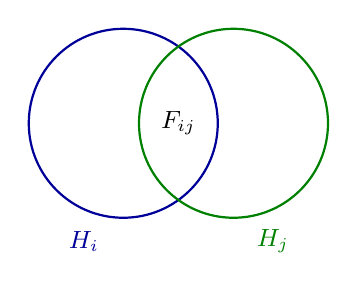
\begin{tikzpicture}[thick, every node/.style={font=\small}]
            \draw[blue!60!black] (0,0) circle (1.2);
            \draw[green!50!black] (1.4,0) circle (1.2);
            \node at (0.7,0) {$F_{ij}$};
            \node[blue!60!black] at (-0.5,-1.5) {$H_i$};
            \node[green!50!black] at (1.9,-1.5) {$H_j$};
        \end{tikzpicture}
    \end{center}
    \begin{itemize}
        \item \emph{Which \(j\) are dependent.} If \(e(F_{ij}) = 0\), then \(E_i\) and \(E_j\) are determined by the disjoint edge sets \(E(H_i)\) and \(E(H_j)\), so they are independent. If \(e(F_{ij}) \ge 1\), then \(E_i \cap E_j\) says that all \(\abs{E(H_i) \cup E(H_j)} = 2e - e(F_{ij})\) edges are present, so for \(0 < p < 1\)
        \[
            \mathbb{P}(E_i \cap E_j) = p^{2e - e(F_{ij})} > p^{2e} = \mathbb{P}(E_i)\,\mathbb{P}(E_j).
        \]
        So \(j \sim i\) iff \(H_i\) and \(H_j\) share an edge, and then
        \begin{equation}\label{eq:subgraph-cond-prob}
            \mathbb{P}(E_j \mid E_i) = \frac{\mathbb{P}(E_i \cap E_j)}{\mathbb{P}(E_i)} = \frac{p^{2e - e(F_{ij})}}{p^{e}} = p^{e - e(F_{ij})}.
        \end{equation}
        \item \emph{\(F_{ij}\) is a proper subgraph of \(H\).} \(F_{ij} \subseteq H_i \cong H\). If \(F_{ij} = H_i\), then \(V(H_i) \subseteq V(H_j)\) and \(E(H_i) \subseteq E(H_j)\); both sides have the same sizes \(v\) and \(e\), so \(H_i = H_j\), contradicting \(j \ne i\). Hence for \(j \sim i\), \(F_{ij}\) is isomorphic to a proper subgraph of \(H\) with at least one edge. Let
        \[
            \mathcal{F} \coloneqq \bigl\{ F \subsetneq H : e(F) \ge 1 \bigr\} \big/ \cong
        \]
        be the set of \emph{isomorphism classes} of such subgraphs, with one representative \(F\) chosen from each class. So \(F \in \mathcal{F}\) is an unlabelled shape: it records the structure of the intersection, not which vertices of \(H_i\) it occupies. \(\mathcal{F}\) is finite and depends only on \(H\).
        \item \emph{Number of \(j\) with \(F_{ij} \cong F\).} Since \(F\) only fixes the shape of \(F_{ij}\), first choose the vertex set of \(F_{ij}\) inside \(V(H_i)\) (at most \(2^{v}\) subsets), then the other \(v - v(F)\) vertices of \(H_j\) (at most \(n^{v - v(F)}\) ways), then the copy of \(H\) on these \(v\) vertices (at most \(v!\) bijections from \(V(H)\)). Every \(j\) with \(F_{ij} \cong F\) arises from some such choice; many choices do not give \(F_{ij} \cong F\), but we only need an upper bound:
        \[
            \#\bigl\{ j : F_{ij} \cong F \bigr\} \le 2^{v} \cdot n^{v - v(F)} \cdot v! .
        \]
    \end{itemize}
    Each \(j \sim i\) has \(F_{ij}\) in exactly one class of \(\mathcal{F}\), so the sets \(\{j : F_{ij} \cong F\}\), \(F \in \mathcal{F}\), partition \(\{j : j \sim i\}\). On the part for \(F\), every term equals \(p^{e - e(F)}\) by \eqref{eq:subgraph-cond-prob}, since \(e(F_{ij}) = e(F)\) for isomorphic graphs. Hence, using the count,
    \[
        \begin{aligned}
            \Delta^{*}
            = \sum_{j \,:\, j \sim i} \mathbb{P}(E_j \mid E_i)
            &= \sum_{F \in \mathcal{F}} \ \sum_{j \,:\, F_{ij} \cong F} p^{e - e(F)}
            \le \sum_{F \in \mathcal{F}} 2^{v}\, v!\, n^{v - v(F)} p^{e - e(F)} \\
            &= \underbrace{2^{v}\, v!\, n^{v} p^{e}}_{\Theta(\mathbb{E}[X_H])} \sum_{F \in \mathcal{F}} n^{-v(F)} p^{-e(F)} ,
        \end{aligned}
    \]
    where \(2^{v} v!\, n^{v} p^{e} = \Theta(M p^{e}) = \Theta(\mathbb{E}[X_H])\) by \(M = \Theta(n^{v})\) and \eqref{eq:subgraph-mean-M}. So it suffices to show
    \begin{equation}\label{eq:subgraph-suffices}
        \sum_{F \in \mathcal{F}} n^{-v(F)} p^{-e(F)} = o(1).
    \end{equation}
    Since \(p \gg n^{-v/e}\), for large \(n\) we may write \(p = n^{-c}\) with \(c = c(n) \le \frac{v}{e} = \frac{1}{m(H)}\). For \(F \in \mathcal{F}\),
    \[
        n^{-v(F)} p^{-e(F)} = n^{-v(F)} n^{c\,e(F)} = n^{c\,e(F) - v(F)} = \Bigl( n^{c \frac{e(F)}{v(F)} - 1} \Bigr)^{v(F)} .
    \]
    As \(H\) is strictly balanced and \(F \subsetneq H\), \(\frac{e(F)}{v(F)} < \frac{e}{v}\), so
    \[
        c\,\frac{e(F)}{v(F)} - 1 \le \frac{v}{e} \cdot \frac{e(F)}{v(F)} - 1 \eqqcolon -\varepsilon_F < 0,
        \qquad\text{hence}\qquad
        n^{-v(F)} p^{-e(F)} \le n^{-\varepsilon_F v(F)} = o(1).
    \]
    \(\mathcal{F}\) is finite, so summing gives \eqref{eq:subgraph-suffices}. Thus \(X_H = (1+o(1))\,\mathbb{E}[X_H]\) with high probability, and in particular \(X_H \ge 1\).
\end{proof}

\begin{remark}\label{rmk:subgraph-threshold-general}
    \(p^{*} = n^{-1/m(H)}\) is the threshold for every \(H\) with \(e(H) \ge 1\), but the proof of \autoref{thm:subgraph-threshold} needs a little more work when \(H\) is not strictly balanced. The \(0\)-statement is \autoref{prop:subgraph-sparse-m}. For the \(1\)-statement, let \(p \gg n^{-1/m(H)}\), so \(n p^{m(H)} = \bigl( n^{1/m(H)} p \bigr)^{m(H)} \to \infty\). Strict balance was only used to prove \eqref{eq:subgraph-suffices}; instead use \(\frac{e(F)}{v(F)} \le m(H)\) (\autoref{def:max-density}) and \(p \le 1\):
    \[
        n^{-v(F)} p^{-e(F)} = \Bigl( n\,p^{\frac{e(F)}{v(F)}} \Bigr)^{-v(F)} \le \bigl( n\,p^{m(H)} \bigr)^{-v(F)} = o(1).
    \]
    Also \(\mathbb{E}[X_H] \to \infty\): by \eqref{eq:subgraph-mean-M}, \(M = \Theta(n^{v(H)})\), \(\frac{e(H)}{v(H)} \le m(H)\) and \(p \le 1\),
    \[
        \mathbb{E}[X_H] = M p^{e(H)} = \Theta\Bigl( \bigl( n\, p^{\frac{e(H)}{v(H)}} \bigr)^{v(H)} \Bigr) \ge \Theta\Bigl( \bigl( n\, p^{m(H)} \bigr)^{v(H)} \Bigr) = \omega(1).
    \]
\end{remark}

\section{Unique-Sum Sets}\label{sec:unique-sums}

\begin{definition}[Unique sums]\label{def:unique-sums}
    A set \(S \subseteq [n]\) has \vocab{unique sums} if no two distinct subsets of \(S\) have the same sum, i.e.\ \(A \mapsto \sum_{s \in A} s\) is injective on subsets \(A \subseteq S\).
\end{definition}

\begin{eg}\label{eg:unique-sums}
    \(\{1,2,3,4\}\) does not have unique sums, because \(1 + 4 = 2 + 3\) and \(1 + 3 = 4\). On the other hand, \(1 + 3 = 2 + 2\) is not an obstruction: \(\{2,2\}\) is not a subset, as each element is used at most once.
\end{eg}

\begin{question}\label{q:unique-sums}
    How large can \(S \subseteq [n]\) be if \(S\) has unique sums?
\end{question}

\emph{Lower bound.} \(S = \{1, 2, 4, 8, \ldots, 2^{\lfloor \log_2 n \rfloor}\} \subseteq [n]\) has unique sums, since \(\sum_{s \in A} s\) has binary digit \(1\) exactly at the positions in \(A\); so \(\abs{S} = \lfloor \log_2 n \rfloor + 1 \ge \log_2 n\) is possible.

\begin{conjecture}[Erd\H{o}s]\label{conj:unique-sums}
    There is a constant \(C > 0\) such that if \(S \subseteq [n]\) has unique sums, then \(\abs{S} \le \log_2 n + C\).
\end{conjecture}

\begin{lemma}[Counting bound]\label{lem:unique-sums-trivial}
    Let \(n \ge 4\). If \(S \subseteq [n]\) has unique sums, then \(\abs{S} \le 2\log_2 n\) and
    \[
        \abs{S} \le \log_2 n + \log_2 \log_2 n + 1 = \log_2 n + (1 + o(1)) \log_2 \log_2 n .
    \]
\end{lemma}

\begin{proof}
    Let \(m = \abs{S}\). Since \(n \ge 4\), \(\log_2 n \ge 2\) and \(\log_2\log_2 n \ge 1\).

    \emph{Case \(m \le 3\).} Both bounds hold:
    \[
        m \le 3 < 4 \le 2\log_2 n,
        \qquad
        m \le 3 < 2 + 1 + 1 \le \log_2 n + \log_2\log_2 n + 1 .
    \]

    \emph{Case \(m \ge 4\).} The elements of \(S\) are distinct and at most \(n\), so for every \(A \subseteq S\),
    \[
        0 \le \sum_{s \in A} s \le \sum_{s \in S} s \le n + (n-1) + \cdots + (n - m + 1) \le nm - 1 .
    \]
    So the \(2^{m}\) subsets have pairwise distinct sums in \(\{0, 1, \ldots, nm-1\}\), a set of \(nm\) values, and
    \begin{equation}\label{eq:unique-sums-count}
        2^{m} \le nm
        \quad\Longrightarrow\quad
        m \le \log_2 n + \log_2 m .
    \end{equation}
    \begin{itemize}
        \item \emph{First bound.} \(2^{m/2} \ge m\) for \(m \ge 4\), i.e.\ \(\log_2 m \le \frac{m}{2}\). Plugging into \eqref{eq:unique-sums-count},
        \[
            m \le \log_2 n + \frac{m}{2}
            \quad\Longrightarrow\quad
            m \le 2\log_2 n .
        \]
        \item \emph{Second bound.} Taking \(\log_2\) of the first bound,
        \[
            \log_2 m \le \log_2(2\log_2 n) = 1 + \log_2\log_2 n,
        \]
        and plugging this into \eqref{eq:unique-sums-count} gives
        \[
            m \le \log_2 n + \log_2\log_2 n + 1 . \qedhere
        \]
    \end{itemize}
\end{proof}

The second moment improves the coefficient of \(\log_2\log_2 n\) from \(1\) to \(\frac{1}{2}\).

\begin{proposition}\label{prop:unique-sums}
    If \(S \subseteq [n]\) has unique sums, then \(\abs{S} \le \log_2 n + \bigl( \frac{1}{2} + o(1) \bigr) \log_2 \log_2 n\).
\end{proposition}

\begin{proof}
    Let \(S = \{s_1, \ldots, s_m\}\). Choose \(\varepsilon_1, \ldots, \varepsilon_m \in \{0,1\}\) uniformly and independently, and let \(X \coloneqq \sum_{i=1}^{m} \varepsilon_i s_i\). By \autoref{thm:linearity},
    \[
        \mathbb{E}[X] = \mathbb{E}\Bigl[ \sum_{i=1}^{m} \varepsilon_i s_i \Bigr] = \sum_{i=1}^{m} s_i\, \mathbb{E}[\varepsilon_i] = \frac{1}{2} \sum_{i=1}^{m} s_i \eqqcolon \mu .
    \]
    The \(\varepsilon_i s_i\) are independent, so variances add; with \(\Var(\varepsilon_i) = \frac{1}{2} - \frac{1}{4} = \frac{1}{4}\) and \(s_i \le n\),
    \[
        \Var(X) = \sum_{i=1}^{m} \Var(\varepsilon_i s_i) = \sum_{i=1}^{m} s_i^{2} \Var(\varepsilon_i) = \frac{1}{4} \sum_{i=1}^{m} s_i^{2} \le \frac{1}{4} m n^{2} .
    \]
    \thmref{thm:chebyshev} with \(a = n\sqrt{m}\) gives
    \[
        \mathbb{P}\bigl( \abs{X - \mu} \ge n\sqrt{m} \bigr) \le \frac{\Var(X)}{n^{2} m} \le \frac{mn^{2}}{4 n^{2} m} = \frac{1}{4},
    \]
    so \(X\) lies in the interval \(I \coloneqq (\mu - n\sqrt{m}, \mu + n\sqrt{m})\) with probability at least \(\frac{3}{4}\).
    \begin{center}
        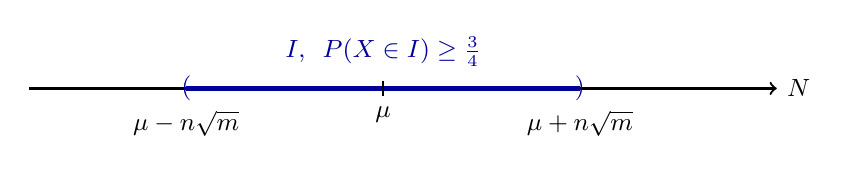
\begin{tikzpicture}[thick, every node/.style={font=\small}]
            \draw[->] (-0.5,0) -- (9,0) node[right] {$\mathbb{N}$};
            \draw[blue!60!black, line width=1.6pt] (1.5,0) -- (6.5,0);
            \node[blue!60!black] at (1.5,0) {$($};
            \node[blue!60!black] at (6.5,0) {$)$};
            \draw (4,0.1) -- (4,-0.1) node[below] {$\mu$};
            \node[below] at (1.5,-0.15) {$\mu - n\sqrt{m}$};
            \node[below] at (6.5,-0.15) {$\mu + n\sqrt{m}$};
            \node[blue!60!black, above] at (4,0.15) {$I$, \ $\mathbb{P}(X \in I) \ge \frac{3}{4}$};
        \end{tikzpicture}
    \end{center}
    The map \((\varepsilon_1, \ldots, \varepsilon_m) \mapsto A = \{s_i : \varepsilon_i = 1\}\) is a bijection \(\{0,1\}^{m} \to \{A \subseteq S\}\), so \(A\) is a uniformly random subset and \(X = \sum_{s \in A} s\). By unique sums, at most one \(A\) has sum \(x\), so \(\mathbb{P}(X = x) \le 2^{-m}\) for every \(x\). As \(X\) is integer-valued and \(I\) contains at most \(2n\sqrt{m} + 1 \le 3n\sqrt{m}\) integers,
    \[
        \frac{3}{4} \le \mathbb{P}(X \in I) = \sum_{x \in I \cap \mathbb{Z}} \mathbb{P}(X = x) \le \frac{3n\sqrt{m}}{2^{m}},
    \]
    so
    \[
        2^{m} \le 4n\sqrt{m}
        \quad\Longrightarrow\quad
        m \le \log_2 n + \frac{1}{2}\log_2 m + 2 .
    \]
    By \autoref{lem:unique-sums-trivial}, \(m \le 2\log_2 n\), so \(\log_2 m \le 1 + \log_2\log_2 n\) and
    \[
        m \le \log_2 n + \frac{1}{2}\log_2\log_2 n + \frac{5}{2} = \log_2 n + \Bigl( \frac{1}{2} + o(1) \Bigr) \log_2\log_2 n . \qedhere
    \]
\end{proof}

The \(2^{m}\) distinct sums occupy \(2^{m}\) distinct integers. \autoref{lem:unique-sums-trivial} only places them in a window of length \(nm\), while \thmref{thm:chebyshev} puts \(\frac{3}{4}\) of them in a window of length \(2n\sqrt{m}\); the saved factor \(\sqrt{m}\) is the saved \(\frac{1}{2}\log_2 m\).

\chapter{The R\"odl Nibble}

\section{Covering \texorpdfstring{\(\ell\)}{l}-Sets by \texorpdfstring{\(k\)}{k}-Sets}\label{sec:covering}

You have \(n\) friends and would like all of them to get along, so you invite them over for dinner, \(k\) at a time.

\begin{question}\label{q:dinner-parties}
    How many dinner parties do we need to host so that every set of \(\ell\) friends has been at the same party together? That is, what is the smallest \(m\) such that there are \(k\)-sets \(S_1, \ldots, S_m \subseteq [n]\) with
    \[
        \forall X \subseteq [n] \text{ with } \abs{X} = \ell, \quad \exists i \text{ such that } X \subseteq S_i \, ?
    \]
\end{question}

\begin{definition}[Covering number, design]\label{def:covering}
    Given \(n \ge k \ge \ell\), let \(M(n,k,\ell)\) be the minimum number of \(k\)-subsets of \([n]\) needed to cover every \(\ell\)-subset of \([n]\) at least once. A \vocab{combinatorial design} is a collection of \(k\)-subsets of \([n]\) such that every \(\ell\)-subset is covered exactly once.
\end{definition}

\begin{proposition}[Counting lower bound]\label{prop:covering-lower}
    \(M(n,k,\ell) \ge \binom{n}{\ell} \big/ \binom{k}{\ell}\), with equality iff a combinatorial design exists.
\end{proposition}

\begin{proof}
    Let \(S_1, \ldots, S_m\) cover every \(\ell\)-set, and count pairs \((X, i)\) with \(\abs{X} = \ell\) and \(X \subseteq S_i\). Each \(S_i\) contains \(\binom{k}{\ell}\) such \(X\), and each of the \(\binom{n}{\ell}\) sets \(X\) lies in at least one \(S_i\):
    \[
        m \binom{k}{\ell} = \#\bigl\{ (X, i) : X \subseteq S_i \bigr\} \ge \binom{n}{\ell} .
    \]
    Equality holds iff every \(X\) lies in exactly one \(S_i\), i.e.\ \(\{S_1, \ldots, S_m\}\) is a design.
\end{proof}

\begin{conjecture}[Erd\H{o}s--Hanani, 1963]\label{conj:erdos-hanani}
    If \(\ell \le k\) are fixed and \(n \to \infty\), then
    \[
        M(n,k,\ell) = (1 + o(1)) \frac{\binom{n}{\ell}}{\binom{k}{\ell}} .
    \]
\end{conjecture}

\begin{theorem}[R\"odl, 1985]\label{thm:rodl}
    \(M(n,k,\ell) = (1 + o(1)) \binom{n}{\ell} \big/ \binom{k}{\ell}\) for fixed \(k \ge \ell\) as \(n \to \infty\).
\end{theorem}

What if we did the most straightforward thing and just chose sets at random? Choose every \(k\)-set \(S\) independently with probability \(p\), and write \(D \coloneqq \binom{n-\ell}{k-\ell}\) for the number of \(k\)-sets containing a fixed \(\ell\)-set. Let
\[
    N \coloneqq \sum_{S \in \binom{[n]}{k}} \mathbbm{1}_{\{S \text{ chosen}\}},
    \qquad
    U \coloneqq \sum_{X \in \binom{[n]}{\ell}} \mathbbm{1}_{\{X \text{ not covered}\}}
\]
be the numbers of chosen \(k\)-sets and of uncovered \(\ell\)-sets.
\begin{itemize}
    \item \emph{Choosing \(p\).} By \autoref{thm:linearity}, \(\mathbb{E}[N] = \binom{n}{k} p\). To match \autoref{prop:covering-lower} we need
    \[
        \binom{n}{k} p \approx \frac{\binom{n}{\ell}}{\binom{k}{\ell}}
        \quad\Longrightarrow\quad
        p \approx \frac{\binom{n}{\ell}}{\binom{n}{k}\binom{k}{\ell}} = \frac{1}{D},
    \]
    using \(\binom{n}{k}\binom{k}{\ell} = \binom{n}{\ell}\binom{n-\ell}{k-\ell}\) (both count pairs \(X \subseteq S \subseteq [n]\) with \(\abs{X} = \ell\), \(\abs{S} = k\)).
    \item \emph{Uncovered \(\ell\)-sets.} An \(\ell\)-set \(X\) is uncovered iff none of the \(D\) \(k\)-sets containing it is chosen, so with \(p = \frac{1}{D}\)
    \[
        \mathbb{P}(X \text{ is not covered}) = (1-p)^{D} \sim e^{-pD} = e^{-1},
    \]
    since \((1 - \frac{1}{D})^{D} \to e^{-1}\) as \(D \to \infty\). By \autoref{thm:linearity}, \(\mathbb{E}[U] \sim e^{-1}\binom{n}{\ell}\).
\end{itemize}
This is \emph{not good enough}: a constant fraction \(e^{-1}\) of the \(\ell\)-sets is left uncovered. Patching each uncovered \(X\) with one extra \(k\)-set containing it gives a cover of expected size
\[
    \mathbb{E}[N + U] \sim \frac{\binom{n}{\ell}}{\binom{k}{\ell}} + e^{-1}\binom{n}{\ell}
    = \Bigl( 1 + e^{-1}\tbinom{k}{\ell} \Bigr) \frac{\binom{n}{\ell}}{\binom{k}{\ell}},
\]
off by a constant factor rather than \(1 + o(1)\). Taking \(p = \frac{t}{D}\) for a constant \(t > 0\) does not help: the same computation gives
\[
    \mathbb{E}[N + U] \sim \Bigl( t + e^{-t}\tbinom{k}{\ell} \Bigr) \frac{\binom{n}{\ell}}{\binom{k}{\ell}},
    \qquad
    t + e^{-t}\tbinom{k}{\ell} \ge t + e^{-t} > 1,
\]
the last step by \(e^{-t} > 1 - t\). So the proof of \autoref{thm:rodl} is not straightforward at all.
